% https://tex.stackexchange.com/questions/428644/
\documentclass[border=5mm]{standalone}
\usepackage{tikz}
\usetikzlibrary{calc}
\usetikzlibrary{arrows.meta}
\begin{document}
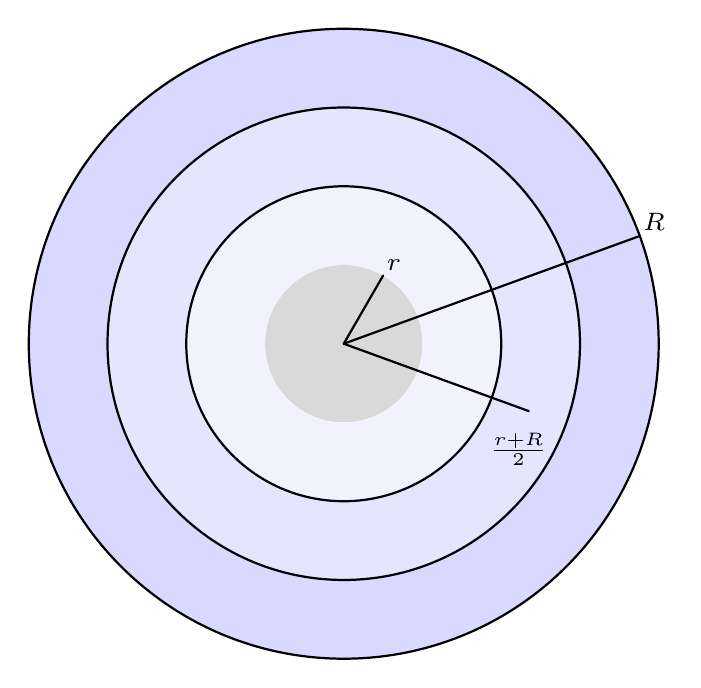
\begin{tikzpicture}[
  line cap=round,
  line join=round,
  >=Triangle,
  myaxis/.style={->,thick},
  every node/.style={scale=1.3}
]

\fill [gray!30] (0,0) circle[radius=1];

%\fill before \draw... repeat loop! (sigh)
\foreach \radius [count=\i] in {2,3,4} {
  \pgfmathsetmacro{\k}{\i * 100/4/5}
  \fill [blue!\k, even odd rule] (0,0) circle[radius=(\radius-1)] circle[radius=\radius];
}
% identical loop as above for the \draw part
\foreach \radius [count=\i] in {2,3,4} {
  \pgfmathsetmacro{\k}{\i * 100/4/5}
  \draw [thick] (0,0) circle[radius=\radius];
}


\begin{scope}[
  every node/.append style={
    circle,
    font=\scriptsize,
    inner sep=1pt
}]
  \draw [thick] (0,0) -- (60:1cm) node[anchor=225] {$r$};
  \draw [thick] (0,0) -- (20:4cm) node[anchor=225] {$R$};
  \draw [thick] (0,0) -- (-20:2.5cm) node[anchor=75] {$\frac{r+R}{2}$};
\end{scope}

\end{tikzpicture}
\end{document}